\begin{minipage}{0.75\linewidth}
\begin{figure}[h]
    \centering
    \begin{adjustbox}{max width=1.0\linewidth, keepaspectratio}
        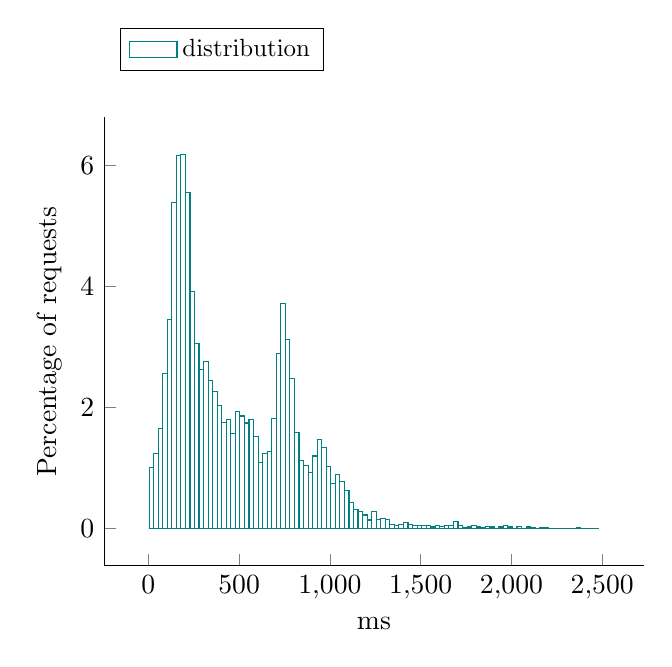
\begin{tikzpicture}
            \begin{axis}[ylabel = Percentage of requests, 
xlabel = ms, 
legend style = {nodes={scale=0.9, transform shape}, at={(0.03,1.2)}, anchor=north west, draw=black, fill=white, align=left, legend columns=3},
area style, mark size = 0pt,
 cycle list name = exotic,
  axis lines* = left]
		\addplot +[ybar interval] coordinates {
			 (4, 1.00766)
			 (29.02, 1.23859)
			 (54.04, 1.64795)
			 (79.06, 2.56114)
			 (104.08, 3.45334)
			 (129.1, 5.3847)
			 (154.12, 6.17193)
			 (179.14, 6.18243)
			 (204.16, 5.56314)
			 (229.18, 3.91519)
			 (254.2, 3.06497)
			 (279.22, 2.63462)
			 (304.24, 2.76058)
			 (329.26, 2.44568)
			 (354.28, 2.26724)
			 (379.3, 2.03632)
			 (404.32, 1.75291)
			 (429.34, 1.7949)
			 (454.36, 1.56398)
			 (479.38, 1.93135)
			 (504.4, 1.85788)
			 (529.42, 1.74242)
			 (554.44, 1.8054)
			 (579.46, 1.52199)
			 (604.48, 1.09163)
			 (629.5, 1.23859)
			 (654.52, 1.27007)
			 (679.54, 1.81589)
			 (704.56, 2.89703)
			 (729.58, 3.72625)
			 (754.6, 3.12795)
			 (779.62, 2.47717)
			 (804.64, 1.58497)
			 (829.66, 1.12312)
			 (854.68, 1.03915)
			 (879.7, 0.923691)
			 (904.72, 1.1966)
			 (929.74, 1.46951)
			 (954.76, 1.34355)
			 (979.78, 1.01816)
			 (1004.8, 0.734754)
			 (1029.82, 0.892201)
			 (1054.84, 0.77674)
			 (1079.86, 0.619293)
			 (1104.88, 0.430356)
			 (1129.9, 0.314895)
			 (1154.92, 0.272909)
			 (1179.94, 0.220426)
			 (1204.96, 0.136454)
			 (1229.98, 0.283405)
			 (1255, 0.146951)
			 (1280.02, 0.157447)
			 (1305.04, 0.146951)
			 (1330.06, 0.0629789)
			 (1355.08, 0.0524824)
			 (1380.1, 0.0629789)
			 (1405.12, 0.0944684)
			 (1430.14, 0.0629789)
			 (1455.16, 0.0524824)
			 (1480.18, 0.0524824)
			 (1505.2, 0.0419859)
			 (1530.22, 0.0524824)
			 (1555.24, 0.020993)
			 (1580.26, 0.0419859)
			 (1605.28, 0.0314895)
			 (1630.3, 0.0419859)
			 (1655.32, 0.0419859)
			 (1680.34, 0.104965)
			 (1705.36, 0.0524824)
			 (1730.38, 0.0104965)
			 (1755.4, 0.020993)
			 (1780.42, 0.0419859)
			 (1805.44, 0.020993)
			 (1830.46, 0.0104965)
			 (1855.48, 0.0314895)
			 (1880.5, 0.020993)
			 (1905.52, 0)
			 (1930.54, 0.020993)
			 (1955.56, 0.0419859)
			 (1980.58, 0.020993)
			 (2005.6, 0)
			 (2030.62, 0.0314895)
			 (2055.64, 0)
			 (2080.66, 0.020993)
			 (2105.68, 0.0104965)
			 (2130.7, 0)
			 (2155.72, 0.0104965)
			 (2180.74, 0.0104965)
			 (2205.76, 0)
			 (2230.78, 0)
			 (2255.8, 0)
			 (2280.82, 0)
			 (2305.84, 0)
			 (2330.86, 0)
			 (2355.88, 0.0104965)
			 (2380.9, 0)
			 (2405.92, 0)
			 (2430.94, 0)
			 (2455.96, 0)
			 (2480.98, 0)
		};
\addlegendentry{distribution};
           \end{axis}
      \end{tikzpicture}
  \end{adjustbox}
  \caption{Response time distribution - req = ReadUser-0}
\end{figure}
\end{minipage}\hfill\begin{minipage}{0.18\linewidth}
\begin{table}[h]
\begin{tabular}{|cc|}
\hline
\textbf{} & \textbf{ms}\\ \hline
 \Xhline{0.005\arrayrulewidth}
min & 4\\
 \Xhline{0.005\arrayrulewidth}
max & 2506\\
 \Xhline{0.005\arrayrulewidth}
mean & 471\\
 \Xhline{0.005\arrayrulewidth}
std & 332\\
\hline
\hline
 \Xhline{0.005\arrayrulewidth}
25th & 194\\
 \Xhline{0.005\arrayrulewidth}
50th & 377\\
 \Xhline{0.005\arrayrulewidth}
75th & 732\\
 \Xhline{0.005\arrayrulewidth}
80th & 767\\
 \Xhline{0.005\arrayrulewidth}
85th & 820\\
 \Xhline{0.005\arrayrulewidth}
90th & 934\\
 \Xhline{0.005\arrayrulewidth}
95th & 1044\\
 \Xhline{0.005\arrayrulewidth}
99th & 1415\\
\hline
\end{tabular}
\caption{Response time}
\end{table}
\end{minipage}\hfill